\documentclass[10pt,aspectratio=169]{beamer}

\usetheme{Madrid}
\usepackage[T1]{fontenc}
\usepackage[utf8]{inputenc}
\usepackage{amsmath,amssymb}
\usepackage{booktabs}
\usepackage{graphicx}
\usepackage{xcolor}

\definecolor{accent}{HTML}{2563EB}
\definecolor{accent2}{HTML}{DC2626}
\definecolor{accent3}{HTML}{059669}
\definecolor{good}{HTML}{059669}
\definecolor{bad}{HTML}{DC2626}

\setbeamercolor{frametitle}{bg=accent,fg=white}
\setbeamertemplate{itemize item}{\textcolor{accent}{$\bullet$}}
\setbeamertemplate{navigation symbols}{}
\setbeamertemplate{footline}[frame number]

\title{Scenario Analysis: Interest Rate Shocks}
\subtitle{Part E(iv) --- MBS Prepayment under Macro Stress}
\author{Yueqi Lin}
\institute{MTH 9877 --- Baruch College, Spring 2026}
\date{May 13, 2026}

% =========================================================================
\begin{document}

% ---- Title ---------------------------------------------------------------
\begin{frame}[plain]
    \titlepage
\end{frame}

% ---- 1. Setup ------------------------------------------------------------
\begin{frame}{TV Cox is the only model with a direct rate channel for scenario analysis.}
    \begin{columns}[T,onlytextwidth]
        \column{0.50\textwidth}
        \begin{block}{Why TV Cox (E(ii)) is the primary model}
        \small
        \texttt{rate\_incentive} $= r_{\text{orig}} - r_{\text{market}}(t)$ is a
        \textbf{direct time-varying covariate}.\\[4pt]
        A $\Delta r$ bp market rate shock immediately shifts the incentive by
        $-\Delta r / 100$\,pp, giving an analytic hazard response:
        \[
            \Delta\log h(t) = \hat\beta_{\text{ri}} \times \frac{-\Delta r}{100}
        \]
        Output: calibrated $S(t)$, CPR, WAL, and price --- all in realistic ranges.
        \end{block}

        \column{0.46\textwidth}
        \begin{alertblock}{Why static DeepCox cannot do this}
        \small
        Static models (Part D) use \texttt{OriginalInterestRate} --- the \textbf{coupon},
        not the market rate.\\[4pt]
        Shocking this field gives the \textbf{wrong economic direction}:
        a rate \emph{cut} reduces the coupon $\Rightarrow$ model predicts \emph{less} prepayment
        (opposite to reality).\\[4pt]
        Static models require architectural changes before scenario analysis is valid.
        \end{alertblock}
    \end{columns}
    \vspace{0.5em}
    \begin{center}
        \small
        Representative loan: \$300K, 6.5\% coupon, baseline market rate 7.0\%.\\
        Scenarios: $\pm$100, $\pm$200, $\pm$300\,bp --- covering the BCBS standard stress range.
    \end{center}
\end{frame}

% ---- 2. Shock sensitivity ------------------------------------------------
\begin{frame}{TV Cox tracks the analytic formula exactly; DeepCox sign is reversed.}
    \begin{center}
        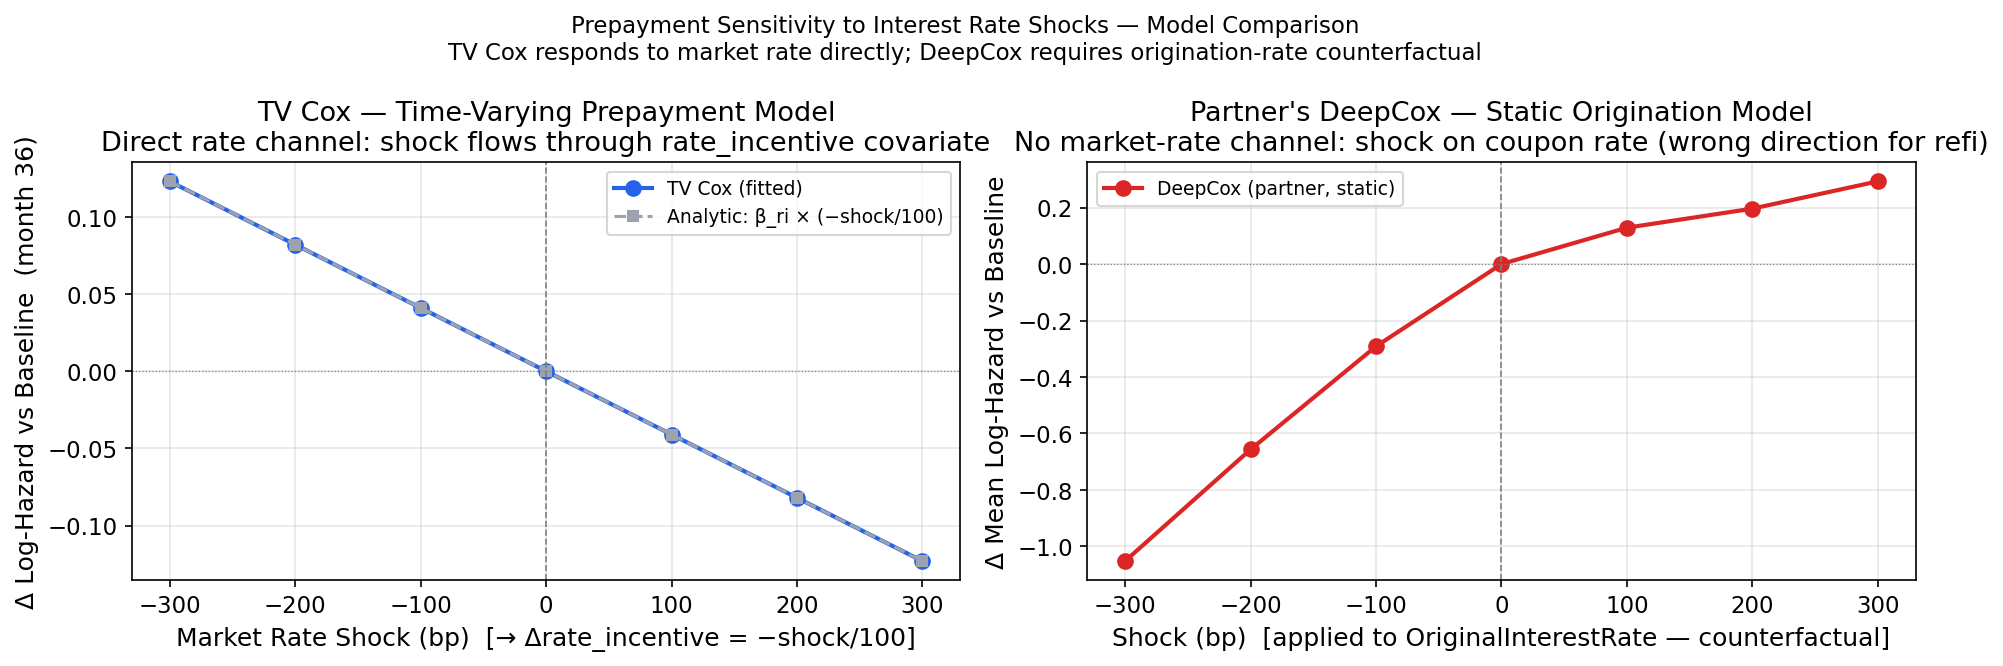
\includegraphics[width=0.88\linewidth]{processed/Eiv_shock_comparison}
    \end{center}
    \vspace{-0.4em}
    \begin{center}
        \small
        \textcolor{accent}{Left}: TV Cox fitted $\Delta\log h$ overlaps the analytic line perfectly
        ($\hat\beta_{\text{ri}} = 0.041$, HR $= 1.042$ per 100\,bp).\\
        \textcolor{bad}{Right}: DeepCox $\Delta\log h$ is \emph{opposite sign} ---
        a 300\,bp cut produces $-1.05$ (less prepayment), not more.
    \end{center}
\end{frame}

% ---- 3. Survival curves --------------------------------------------------
\begin{frame}{Rate scenarios shift survival by 6.7\,pp and median prepayment by 11 months.}
    \begin{columns}[c,onlytextwidth]
        \column{0.62\textwidth}
        \begin{center}
            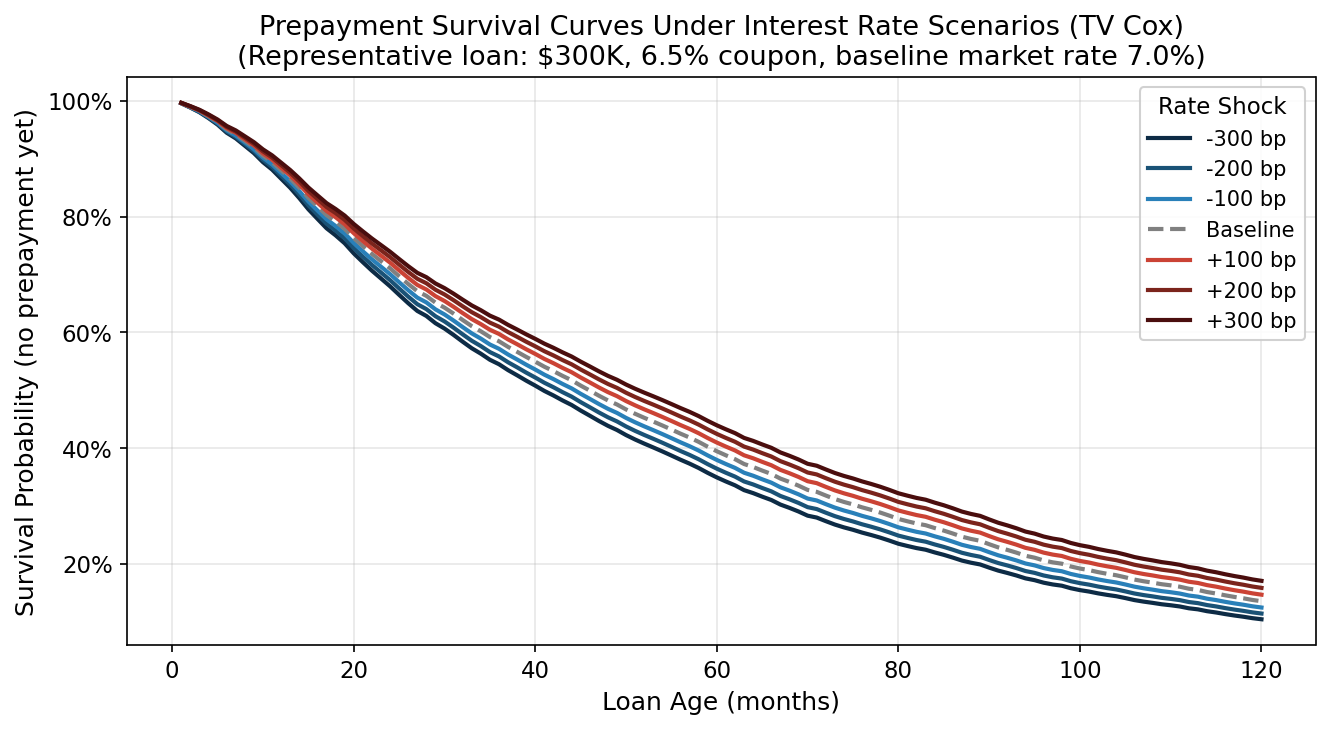
\includegraphics[width=\linewidth]{processed/Eiv_survival_curves}
        \end{center}

        \column{0.34\textwidth}
        \small
        \begin{tabular}{@{}lcc@{}}
            \toprule
            Scenario & 10-yr & Med.~mo. \\
            \midrule
            $-300$\,bp & 10.4\% & 41 \\
            $-200$\,bp & 11.4\% & 43 \\
            $-100$\,bp & 12.5\% & 45 \\
            Baseline   & 13.5\% & 46 \\
            $+100$\,bp & 14.7\% & 48 \\
            $+200$\,bp & 15.8\% & 50 \\
            $+300$\,bp & 17.1\% & 52 \\
            \bottomrule
        \end{tabular}
        \vspace{0.5em}

        \small Curves monotonically ordered.\\
        $\pm300$\,bp: 6.7\,pp survival range,\\
        11-month shift in median prepay.
    \end{columns}
\end{frame}

% ---- 4. S-curve + contour ------------------------------------------------
\begin{frame}{The S-curve is smooth; FICO gates refi access, LTV caps the upside.}
    \begin{columns}[c,onlytextwidth]
        \column{0.50\textwidth}
        \begin{center}
            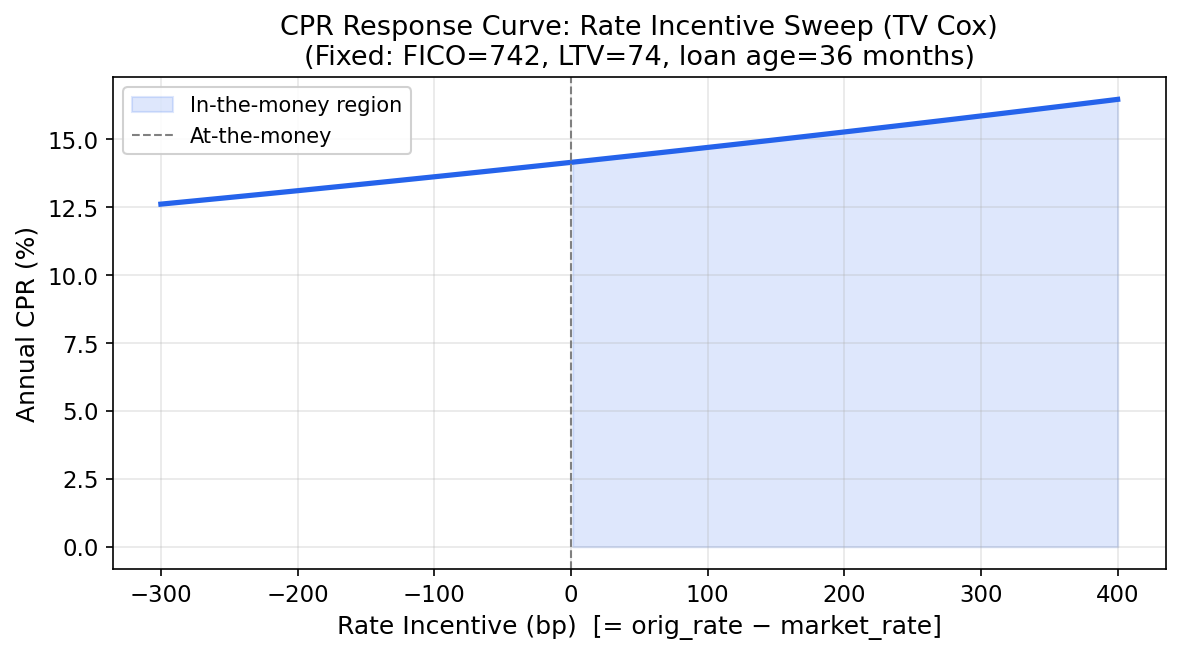
\includegraphics[width=\linewidth]{processed/Eiv_scurve}
        \end{center}
        \vspace{-0.3em}
        \begin{center}
            \small
            CPR: 12.6\% at $-300$\,bp $\to$ 16.5\% at $+400$\,bp.\\
            Flat slope reflects compressed $\hat\beta_{\text{ri}} = 0.041$\\
            (penalizer + 500K-row subsample).
        \end{center}

        \column{0.48\textwidth}
        \begin{center}
            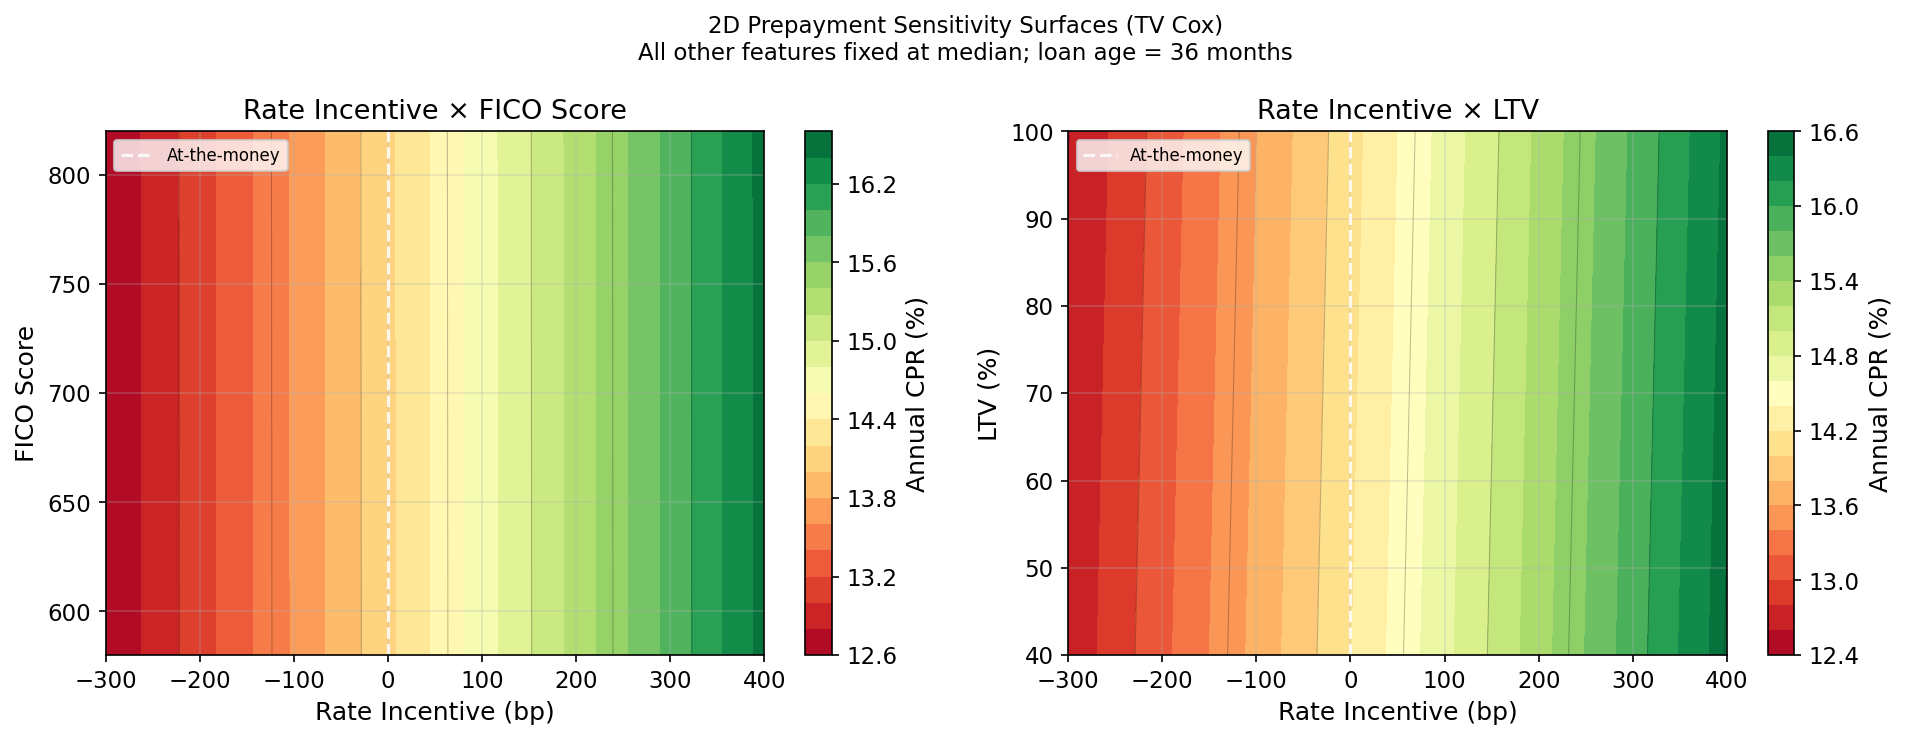
\includegraphics[width=\linewidth]{processed/Eiv_contour}
        \end{center}
        \vspace{-0.3em}
        \begin{center}
            \small
            FICO $>720$: credit access enables refinancing.\\
            LTV $>90$: equity constraint flattens CPR
            regardless of incentive.
        \end{center}
    \end{columns}
\end{frame}

% ---- 5. MBS cash flows ---------------------------------------------------
\begin{frame}{WAL range 0.57\,yr; price range \$17.70 --- negative convexity confirmed.}
    \begin{columns}[c,onlytextwidth]
        \column{0.60\textwidth}
        \begin{center}
            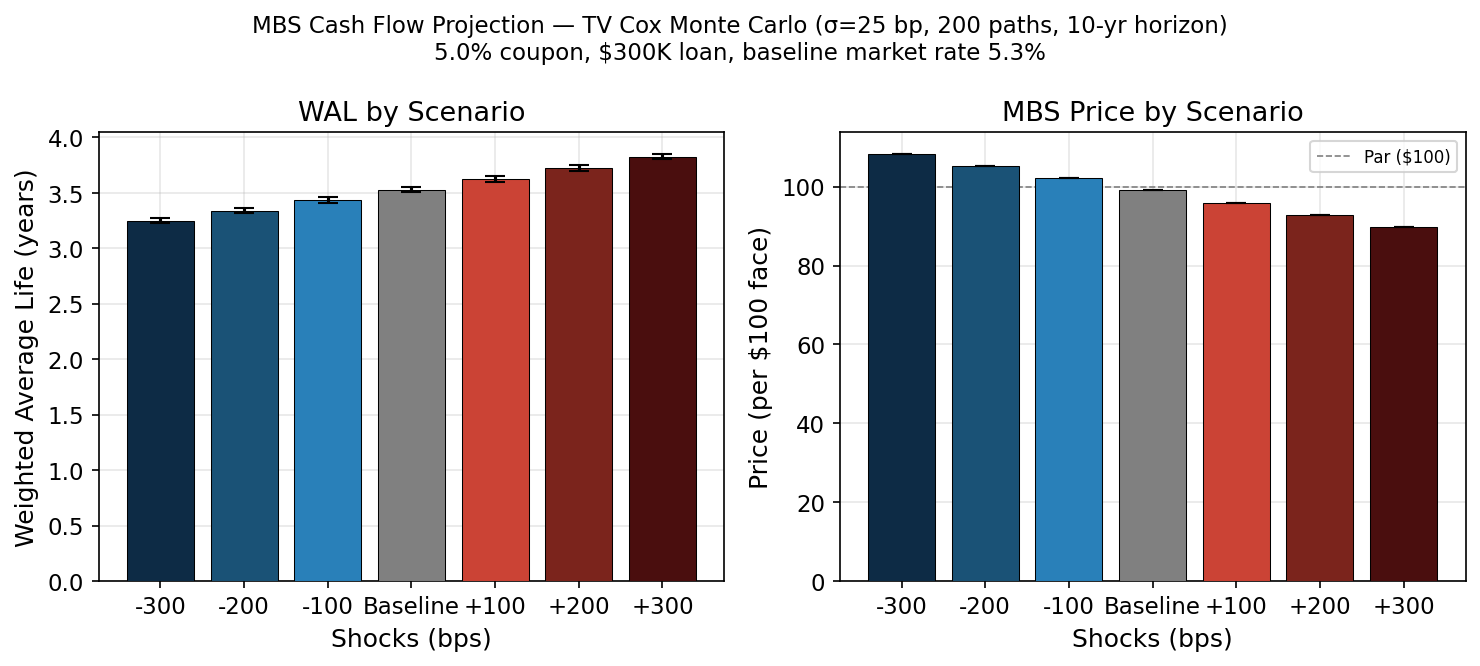
\includegraphics[width=\linewidth]{processed/Eiv_mbs_cashflows}
        \end{center}

        \column{0.36\textwidth}
        \small
        \begin{tabular}{@{}lrr@{}}
            \toprule
            Scenario & WAL & Price\,(\$) \\
            \midrule
            $-300$\,bp & 3.21 & 107.35 \\
            $-200$\,bp & 3.30 & 104.42 \\
            $-100$\,bp & 3.39 & 101.48 \\
            Baseline   & 3.48 & \phantom{0}98.52 \\
            $+100$\,bp & 3.58 & \phantom{0}95.56 \\
            $+200$\,bp & 3.68 & \phantom{0}92.60 \\
            $+300$\,bp & 3.78 & \phantom{0}89.65 \\
            \bottomrule
        \end{tabular}
        \vspace{0.5em}

        \small MC: 200 paths, $\sigma{=}25$\,bp.\\
        Base $<$ par: rate $>$ coupon.\\[4pt]
        $-300$\,bp gain (\$8.83) $<$ $+300$\,bp loss (\$8.87):\\
        \textbf{negative convexity confirmed}.
    \end{columns}
\end{frame}

% ---- 6. Key Takeaways ----------------------------------------------------
\begin{frame}{Key Takeaways}
    \begin{enumerate}\itemsep5pt
        \item \textbf{Time-varying covariates are required for rate scenario analysis}:
              static models produce the wrong sign when the shock variable is a coupon rate,
              not a market rate.
        \item \textbf{TV Cox tracks the analytic formula exactly}:
              $\Delta\log h = \hat\beta_{\text{ri}} \times (-\Delta r/100)$ with
              $\hat\beta_{\text{ri}} = 0.041$ matches fitted values at all seven shock levels.
        \item \textbf{Rate sensitivity is currently compressed}:
              WAL range 0.57\,yr vs.\ 2--10\,yr for agency MBS.
              Root cause: 500K-row subsample (0.7\% of panel) + Ridge penalizer.
              Lower penalizer and larger sample are the two highest-leverage fixes.
        \item \textbf{Negative convexity is captured}: price upside (\$8.83) $<$
              downside (\$8.87) at $\pm$300\,bp, consistent with prepayment curtailing
              price appreciation.
        \item \textbf{FICO gates access; LTV caps the ceiling}:
              2D contour confirms both constraints from E(i) and E(ii) coefficient signs.
    \end{enumerate}
\end{frame}

% ---- Thank you ------------------------------------------------------------
\begin{frame}[plain]
    \vspace*{2em}
    \begin{center}
        {\Huge \textbf{Thank you}}\\[1.5em]
        {\Large Questions?}\\[2.5em]
        \small
        Andersen \& Gill (1982) \textit{Ann.\ Stat.} $\cdot$
        Sadhwani et al.\ (2021) \textit{J.\ Fin.\ Econometrics} $\cdot$
        BCBS (2019) \textit{Interest Rate Risk in the Banking Book}
    \end{center}
\end{frame}

\end{document}
